\chapter{Santiago du Chili}
\section*{11 mars 2015}
Au retour de l'île de Pâques, je retrouve le vélo chez Nelson qui m'héberge 2 nuits de plus. \newline
\centerline{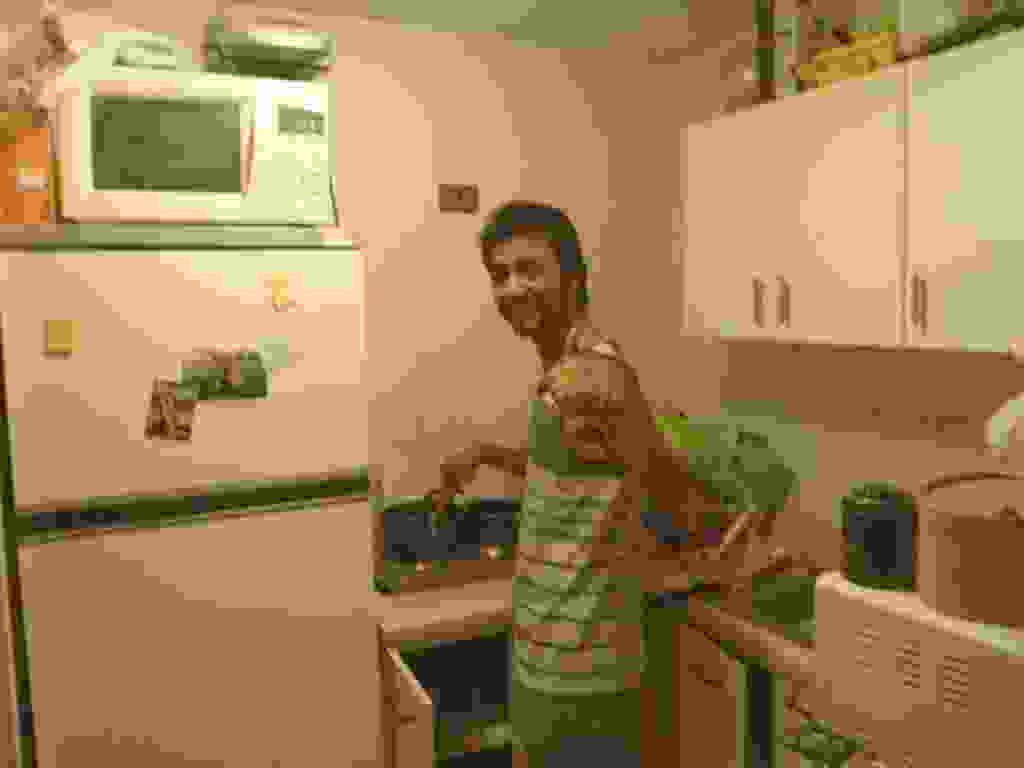
\includegraphics[height=90mm]{../wp-content/uploads/2015/03/P3012432-1024x768.jpg} } 
 Santiago se prête assez bien au vélo, il y a quelques pistes cyclables et des parcs agréables. \newline
\centerline{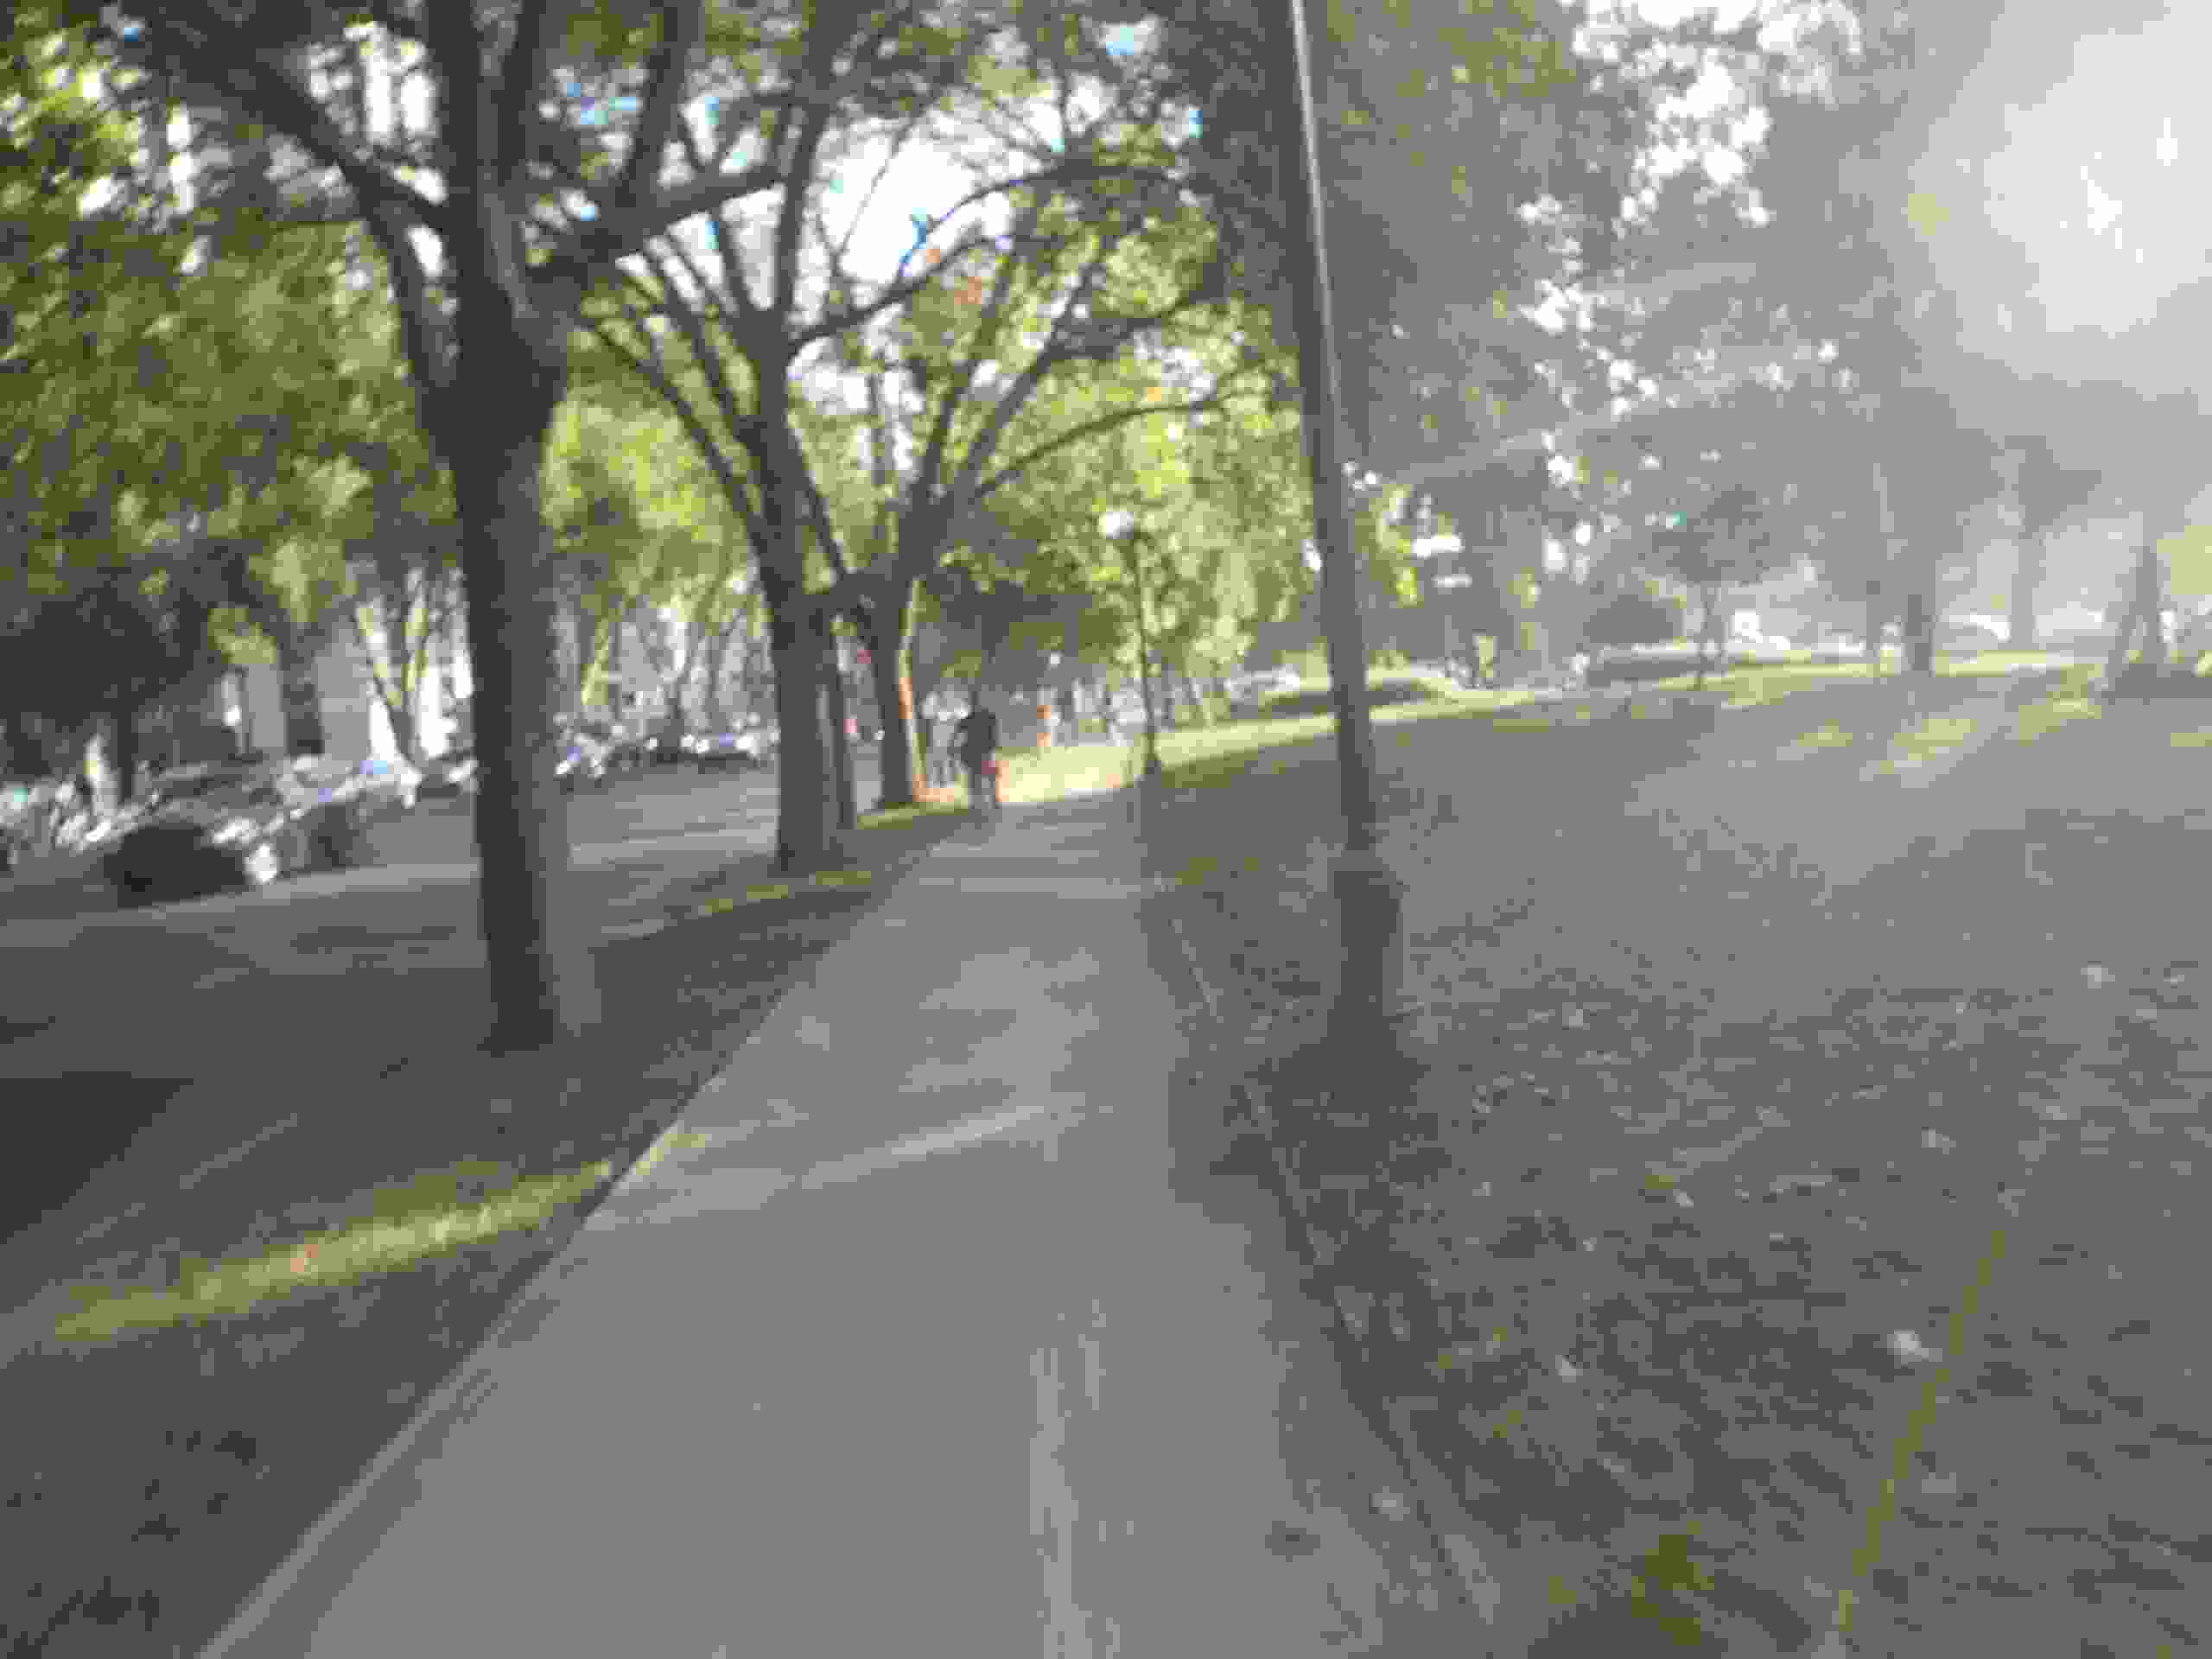
\includegraphics[height=90mm]{../wp-content/uploads/2015/03/P3062599.jpg} } 
 \newline
\centerline{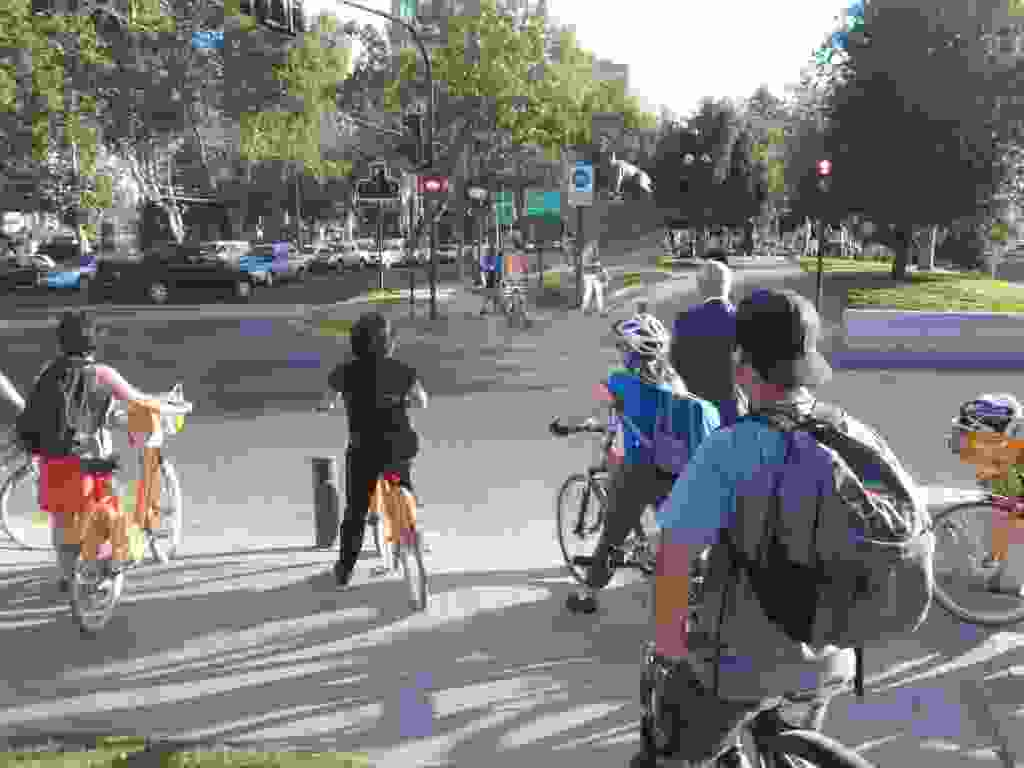
\includegraphics[height=90mm]{../wp-content/uploads/2015/03/P3062598-1024x768.jpg} } 
\newline
\centerline{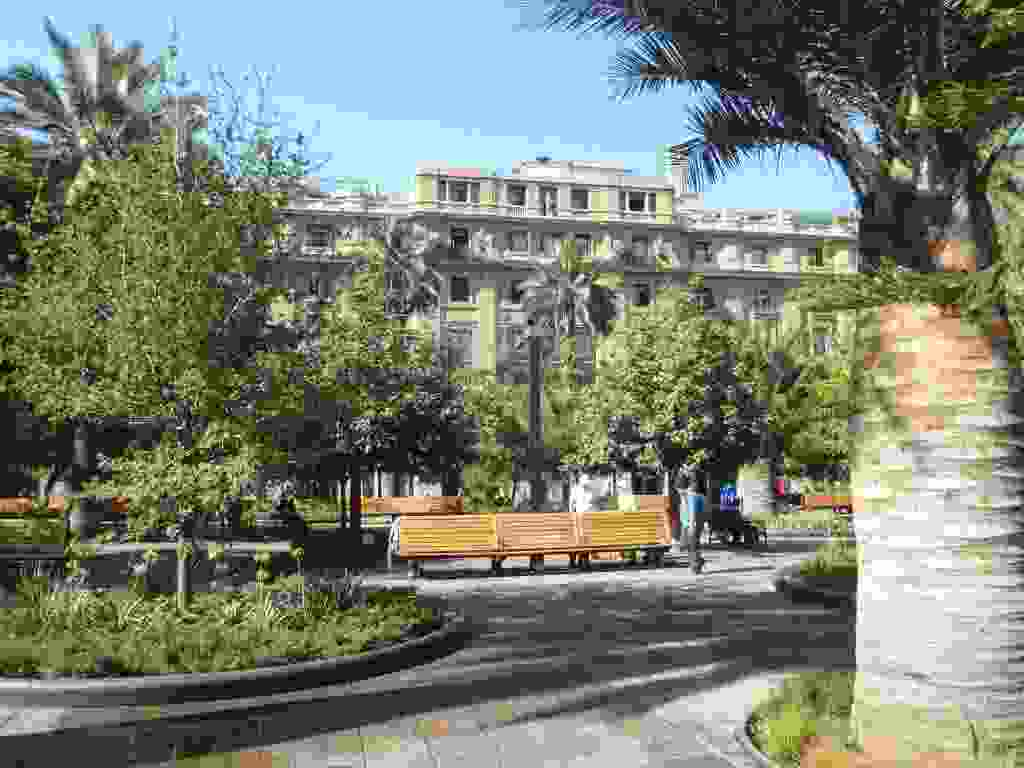
\includegraphics[height=90mm]{../wp-content/uploads/2015/03/P3052566-1024x768.jpg} } 
\newline
\centerline{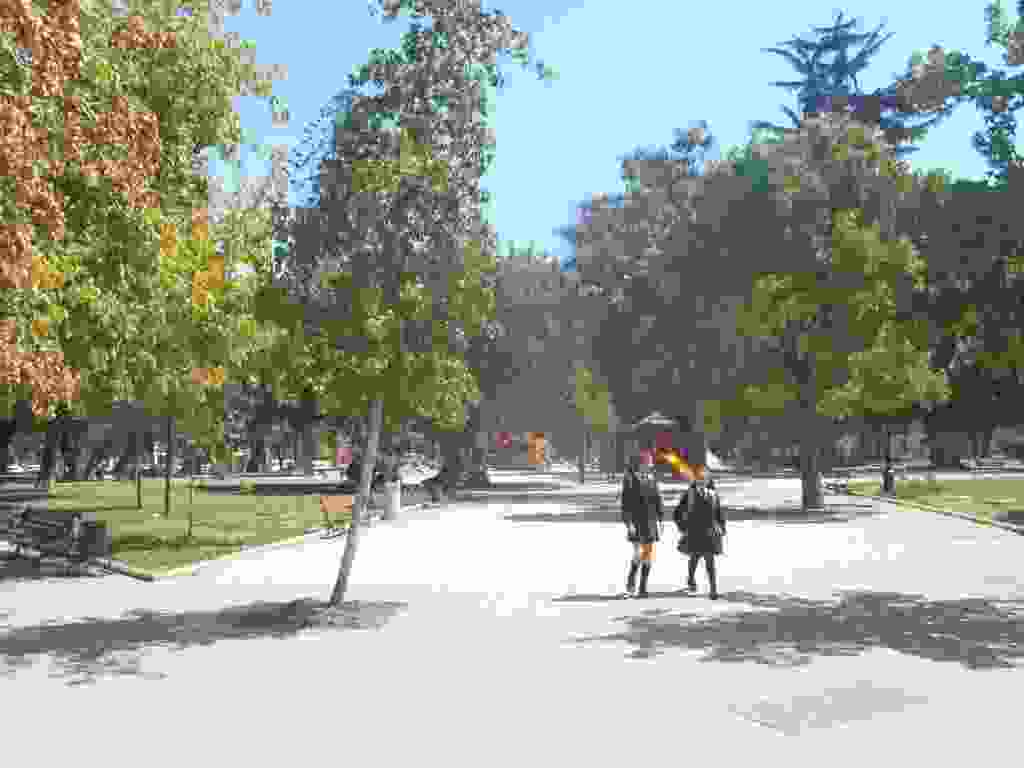
\includegraphics[height=90mm]{../wp-content/uploads/2015/03/P3062617-1024x768.jpg} } 
 Rue piétonne dans le centre.\newline
\centerline{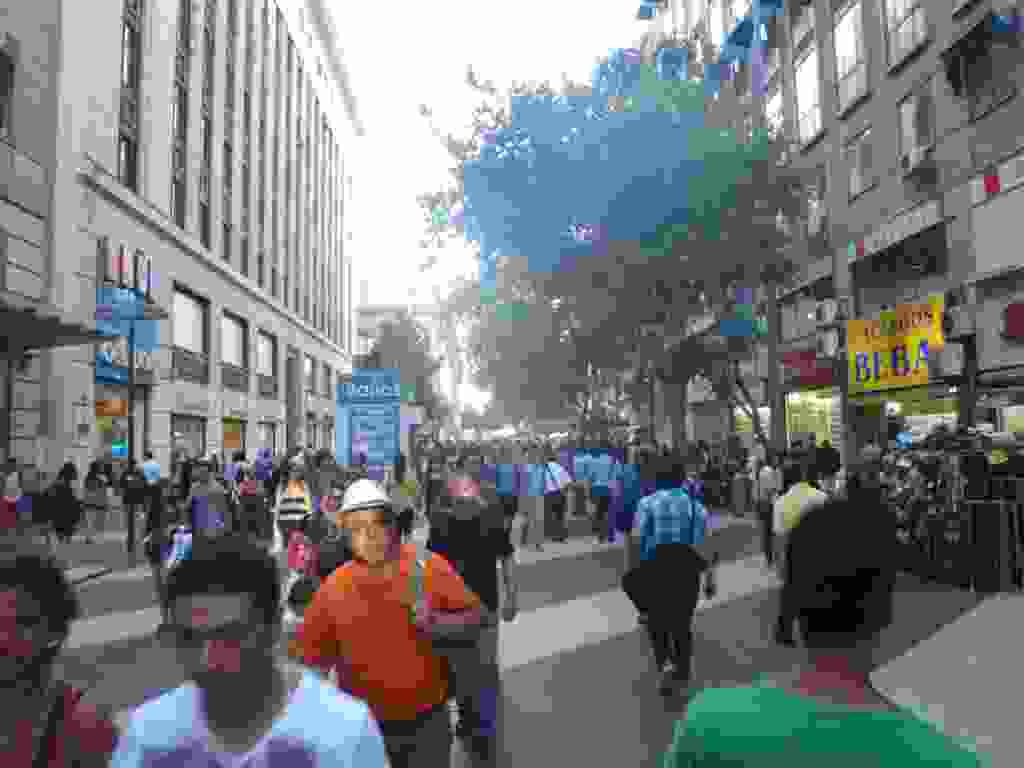
\includegraphics[height=90mm]{../wp-content/uploads/2015/03/P3062630-1024x768.jpg} } 
 Le Palacio de la Moneda, le palais présidentiel. \newline
\centerline{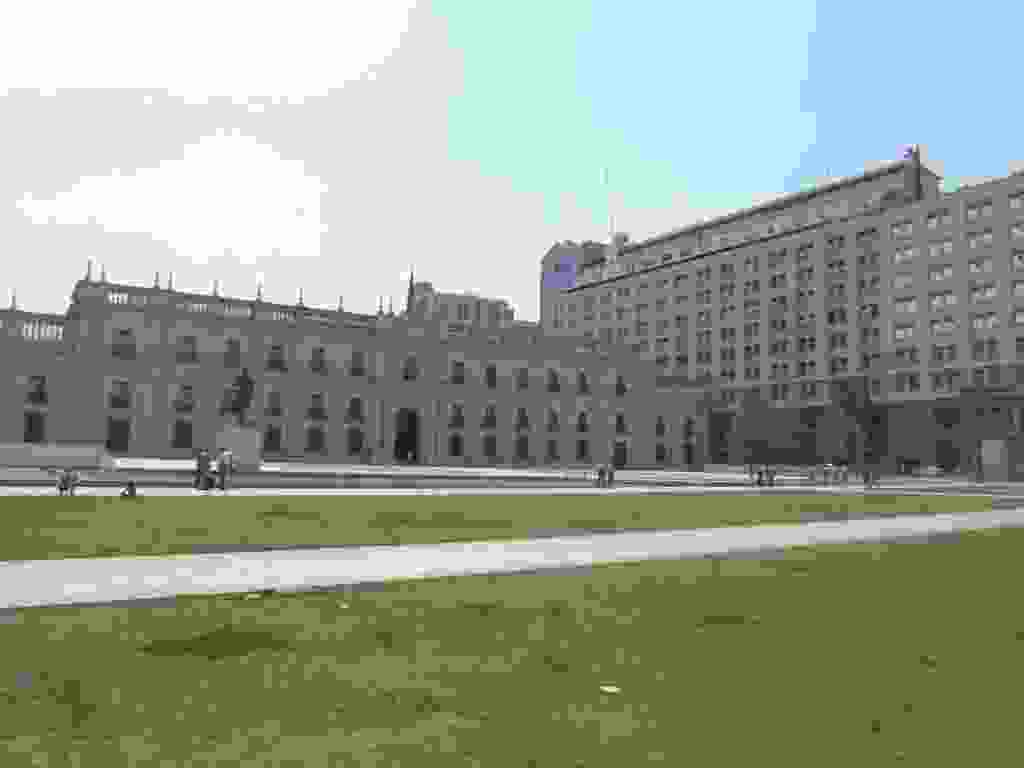
\includegraphics[height=90mm]{../wp-content/uploads/2015/03/P2282423-1024x768.jpg} } 
 \newline
\centerline{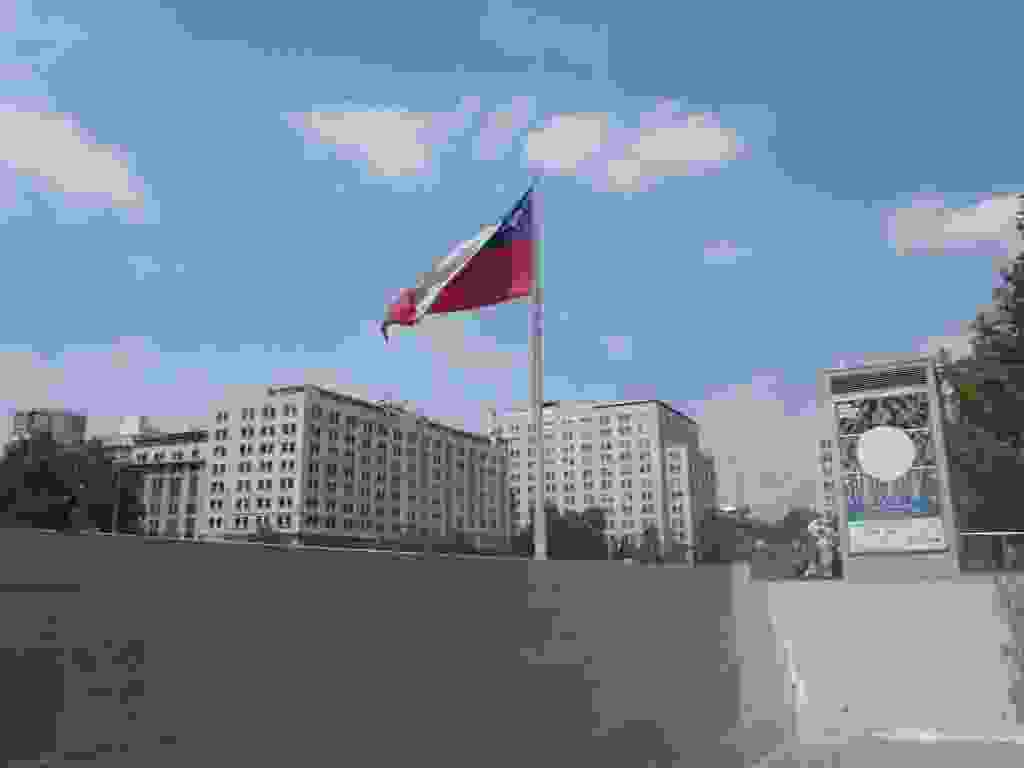
\includegraphics[height=90mm]{../wp-content/uploads/2015/03/P2282424-1024x768.jpg} } 
 \newline
\centerline{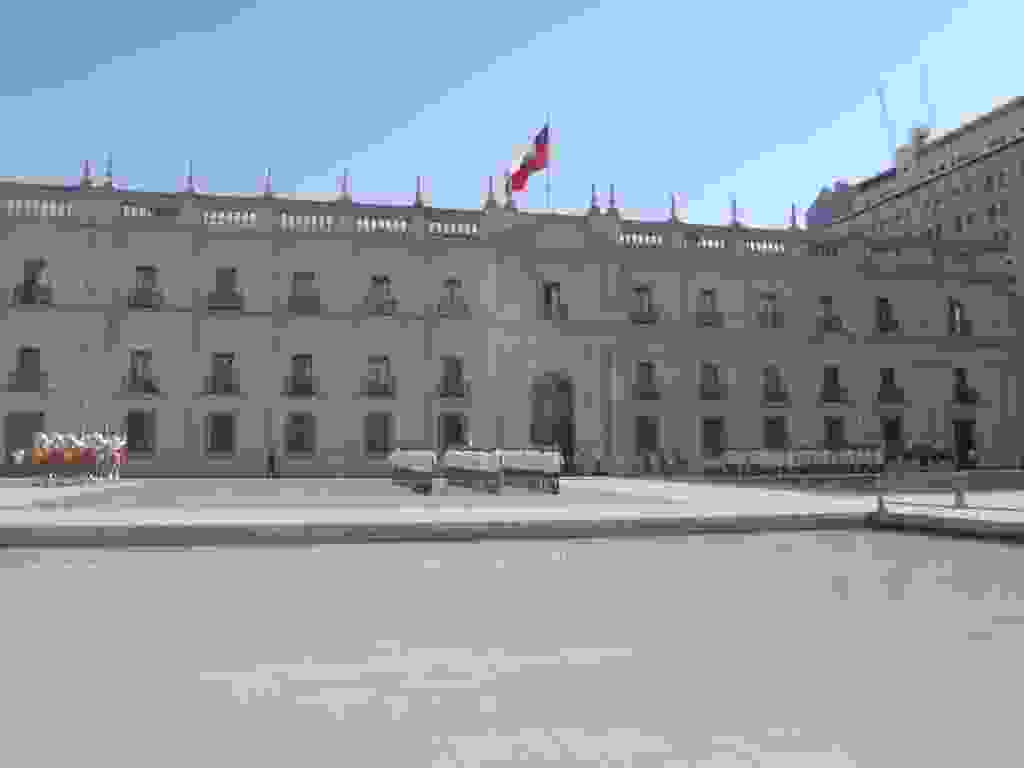
\includegraphics[height=90mm]{../wp-content/uploads/2015/03/P3062612-1024x768.jpg} } 
La colline Santa Lucia qui donne une vue intéressante sur le centre ville. \newline
\centerline{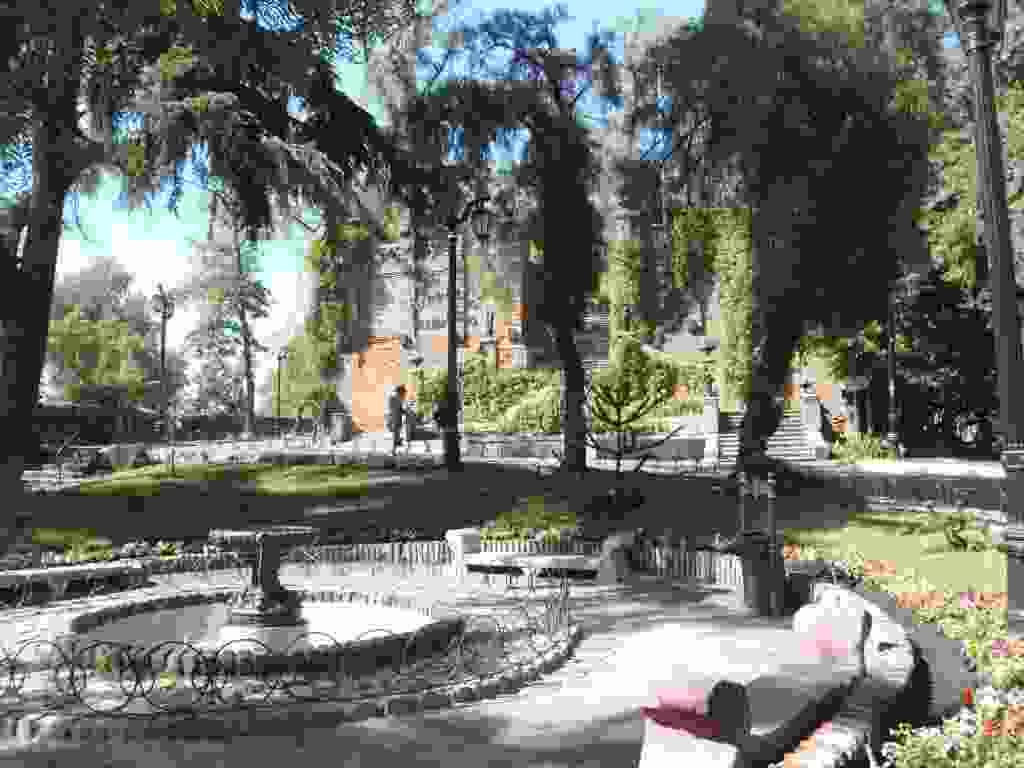
\includegraphics[height=90mm]{../wp-content/uploads/2015/03/P3052571-1024x768.jpg} } 
 \newline
\centerline{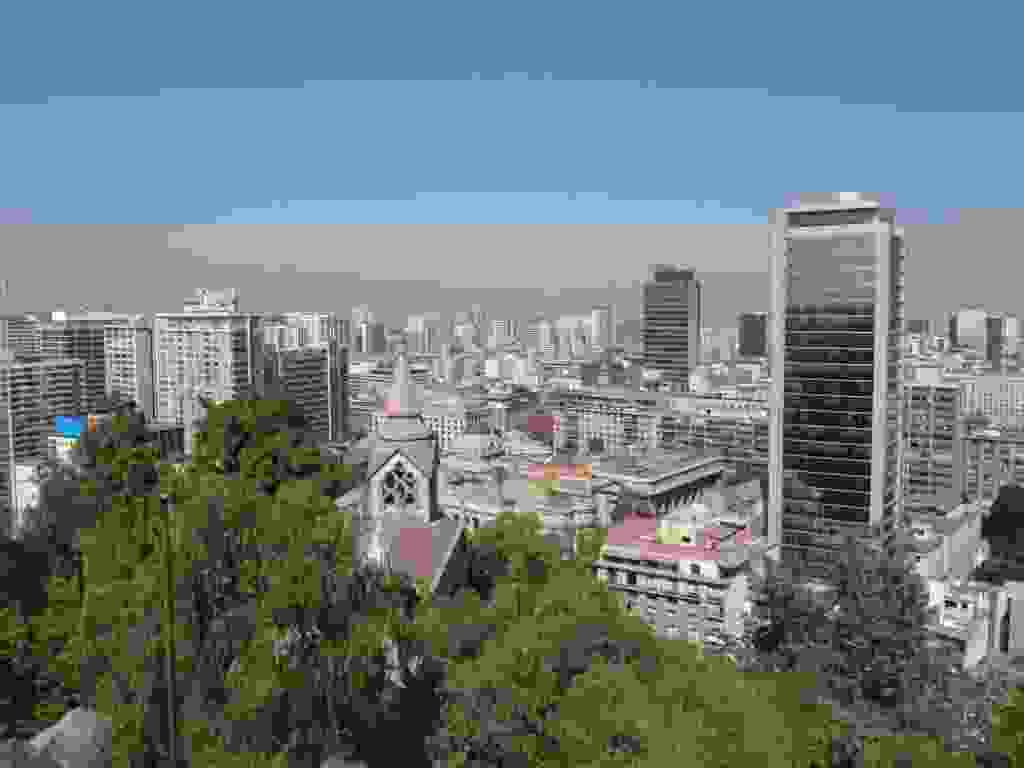
\includegraphics[height=90mm]{../wp-content/uploads/2015/03/P3052573-1024x768.jpg} } 
 \newline
\centerline{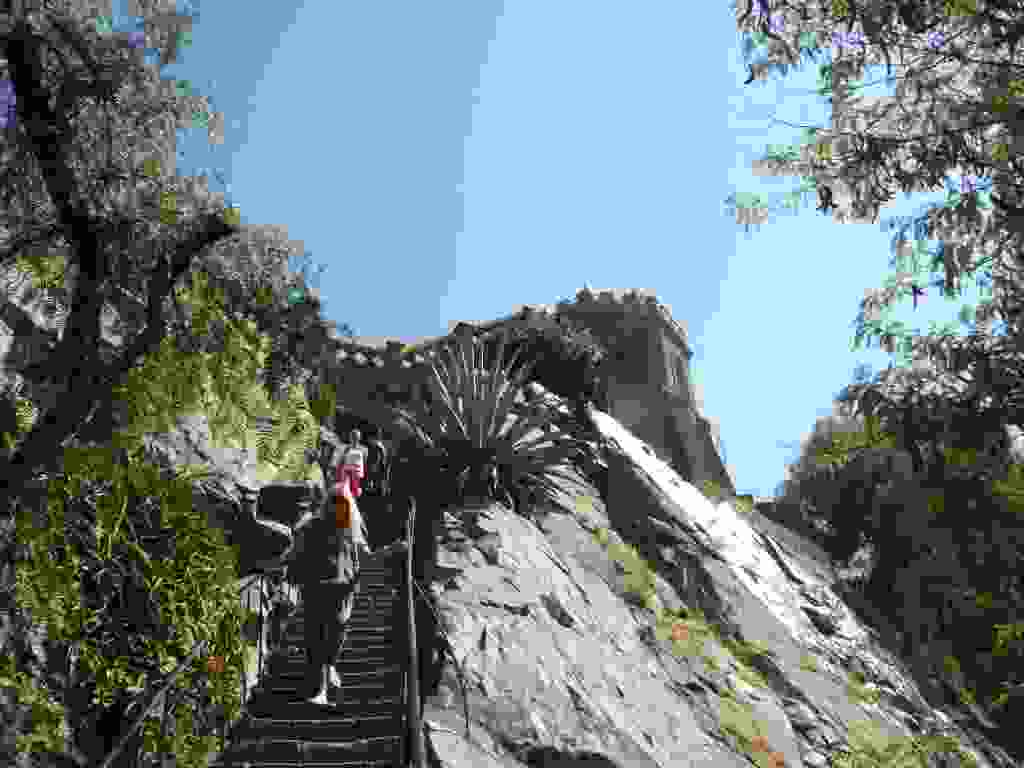
\includegraphics[height=90mm]{../wp-content/uploads/2015/03/P3052578-1024x768.jpg} } 
 \newline
\centerline{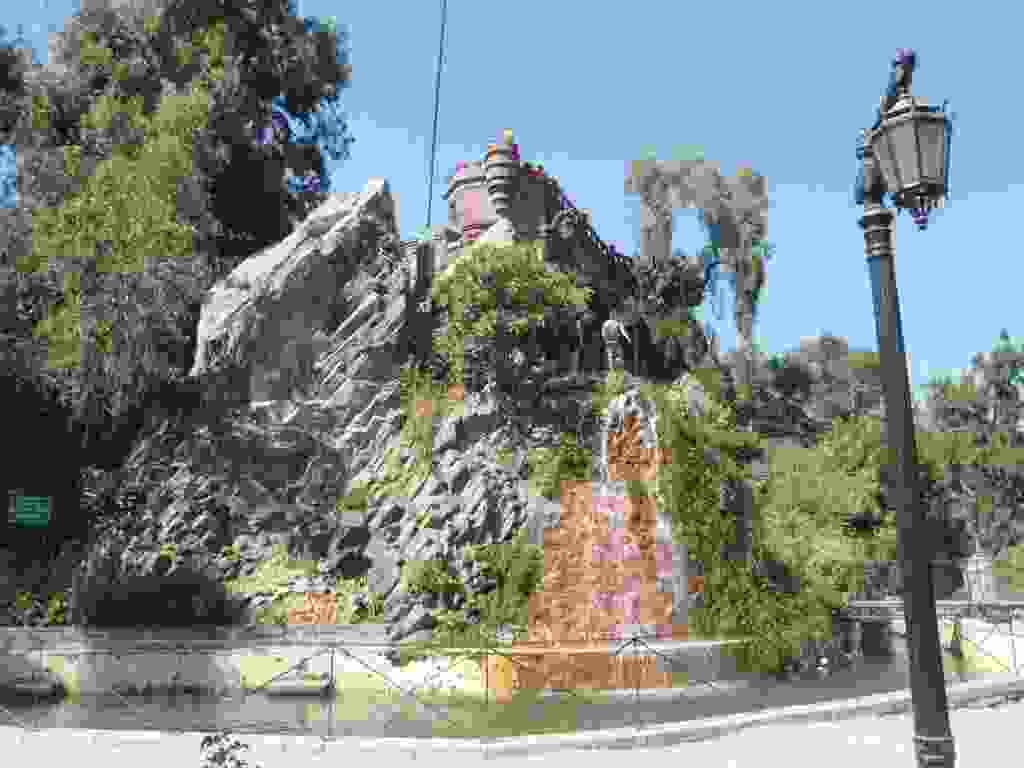
\includegraphics[height=90mm]{../wp-content/uploads/2015/03/P3052580-1024x768.jpg} } 
Le Mercado Central, marché aux poissons. \newline
\centerline{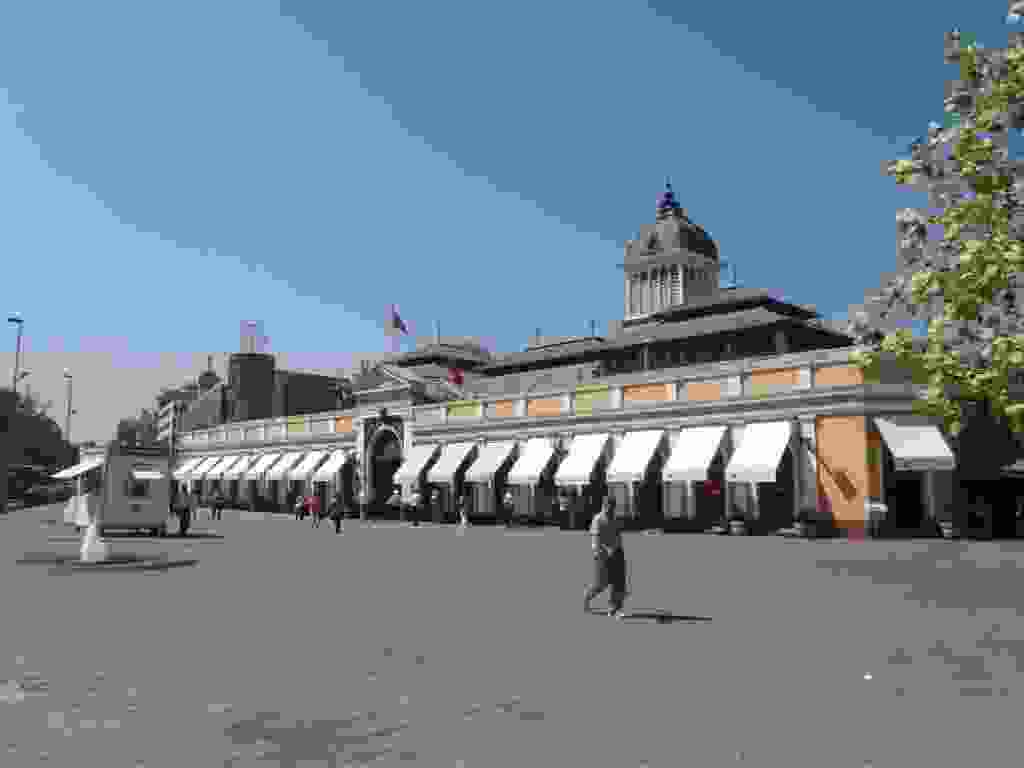
\includegraphics[height=90mm]{../wp-content/uploads/2015/03/P3052583-1024x768.jpg} } 
 \newline
\centerline{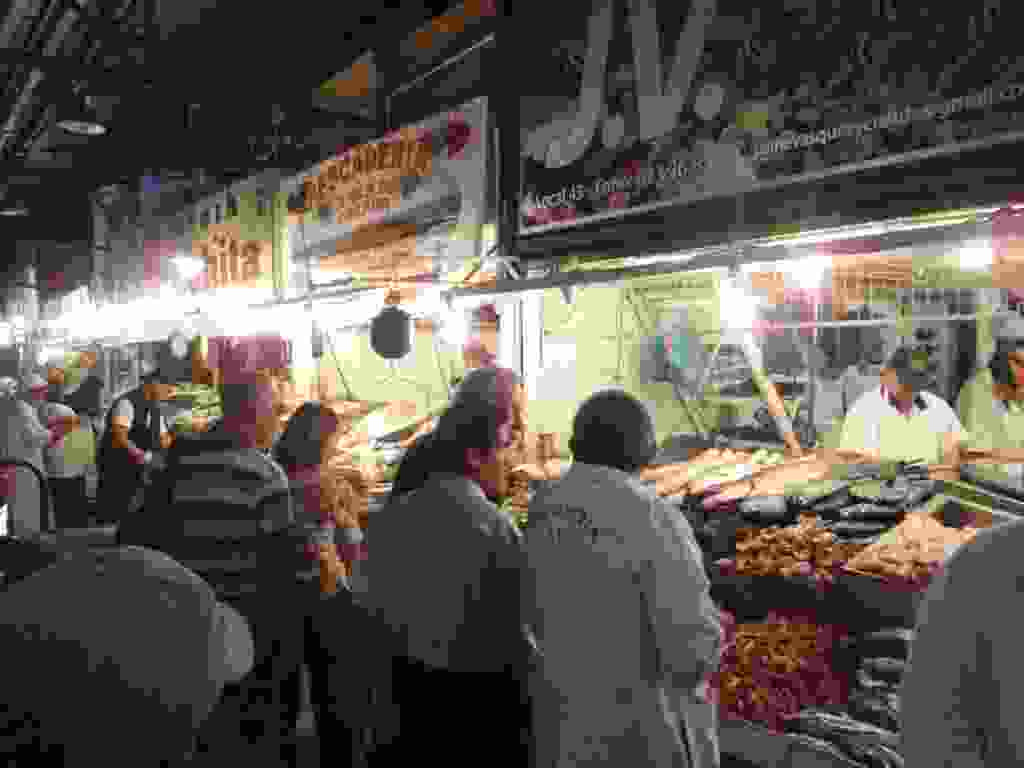
\includegraphics[height=90mm]{../wp-content/uploads/2015/03/P3052584-1024x768.jpg} } 
J'ai goûté à la Paila Marina, une soupe de fruits de mer. \newline
\centerline{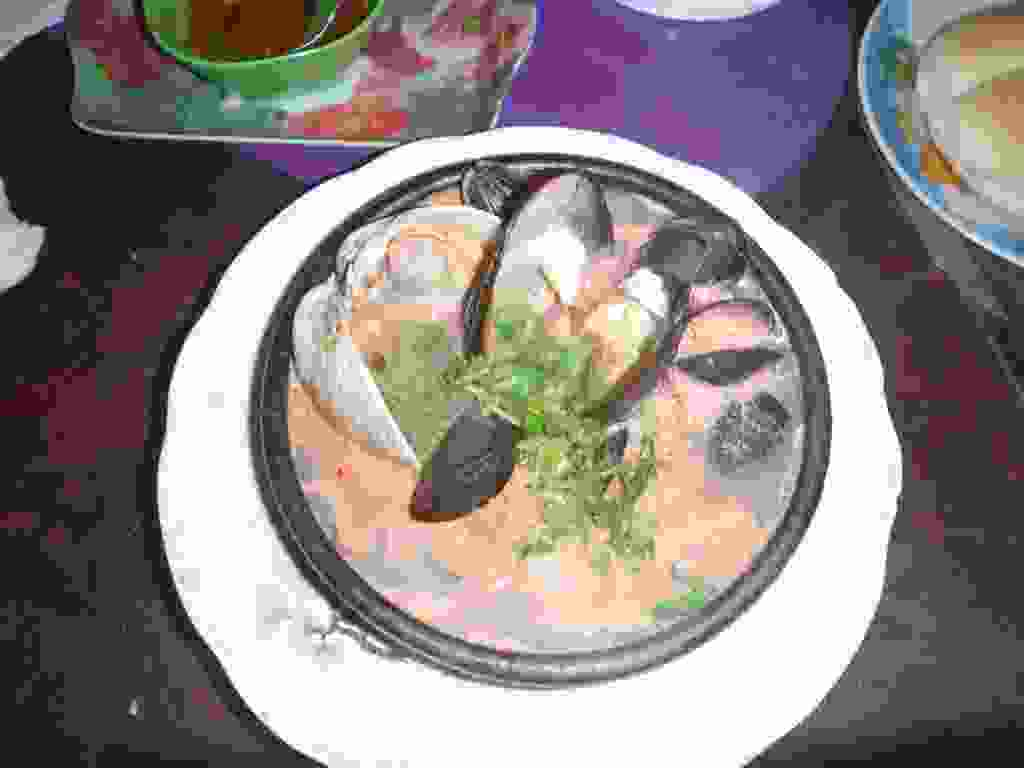
\includegraphics[height=90mm]{../wp-content/uploads/2015/03/P3052587-1024x768.jpg} } 
La colline San Cristobal, immense parc avec une vue encore plus panoramique sur Santiago. On distingue même la cordillère des Andes au loin. \newline
\centerline{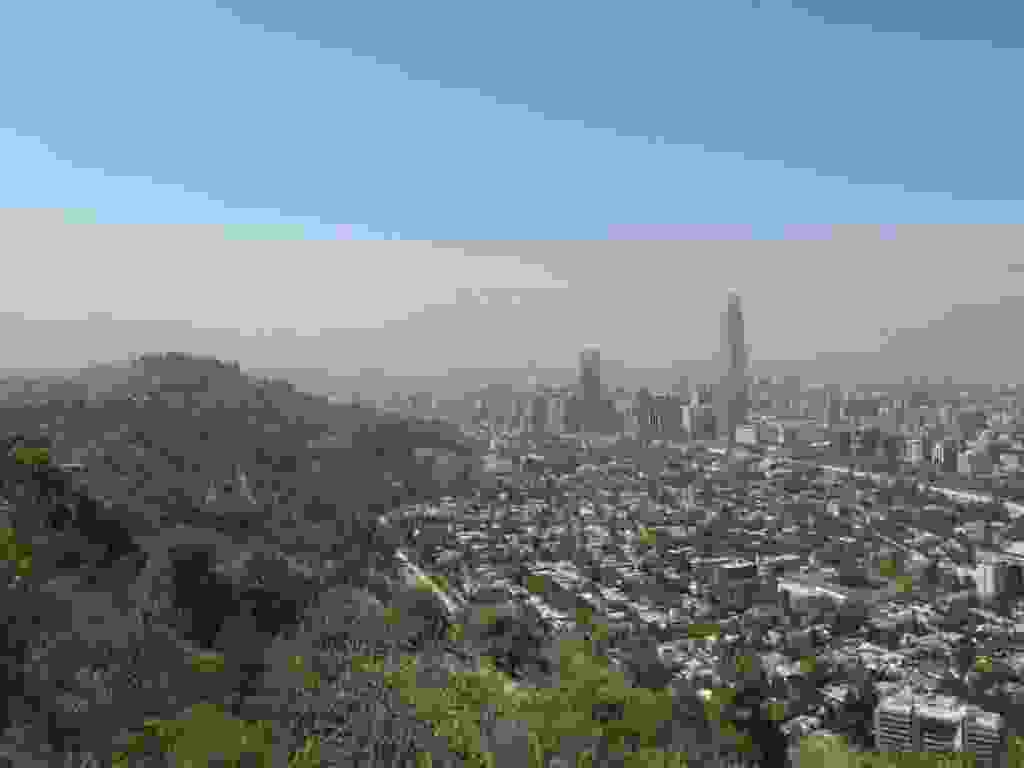
\includegraphics[height=90mm]{../wp-content/uploads/2015/03/P3052588-1024x768.jpg} } 
 \newline
\centerline{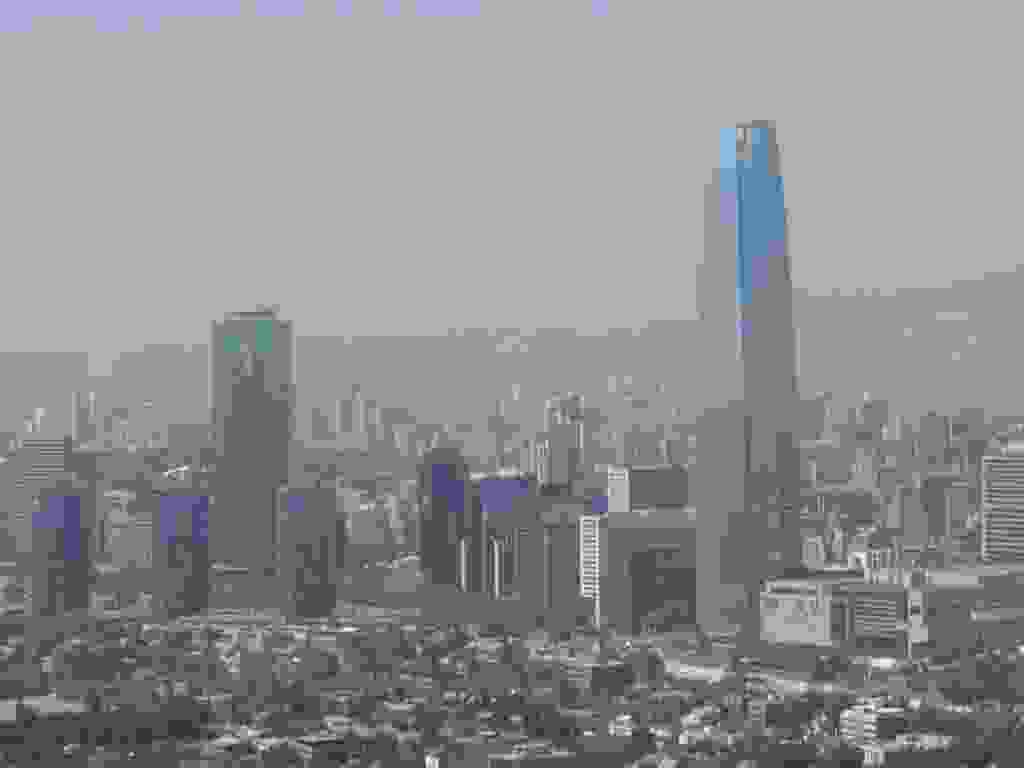
\includegraphics[height=90mm]{../wp-content/uploads/2015/03/P3052589-1024x768.jpg} } 
 \newline
\centerline{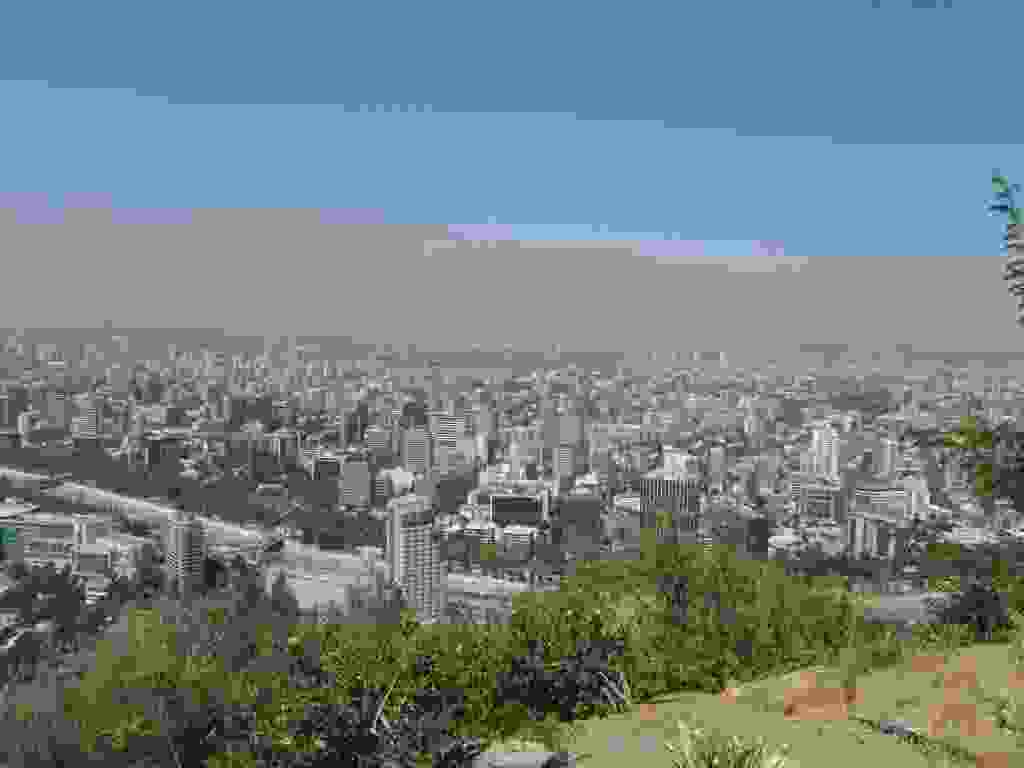
\includegraphics[height=90mm]{../wp-content/uploads/2015/03/P3052590-1024x768.jpg} } 
 \newline
\centerline{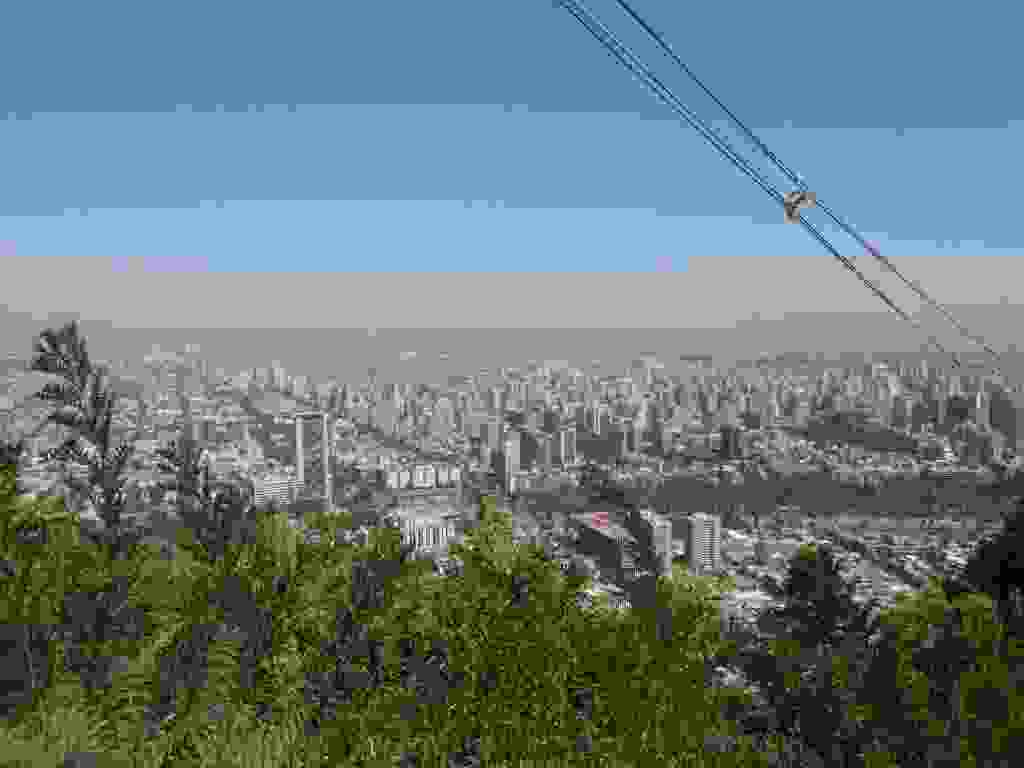
\includegraphics[height=90mm]{../wp-content/uploads/2015/03/P3052591-1024x768.jpg} } 
 \newline
\centerline{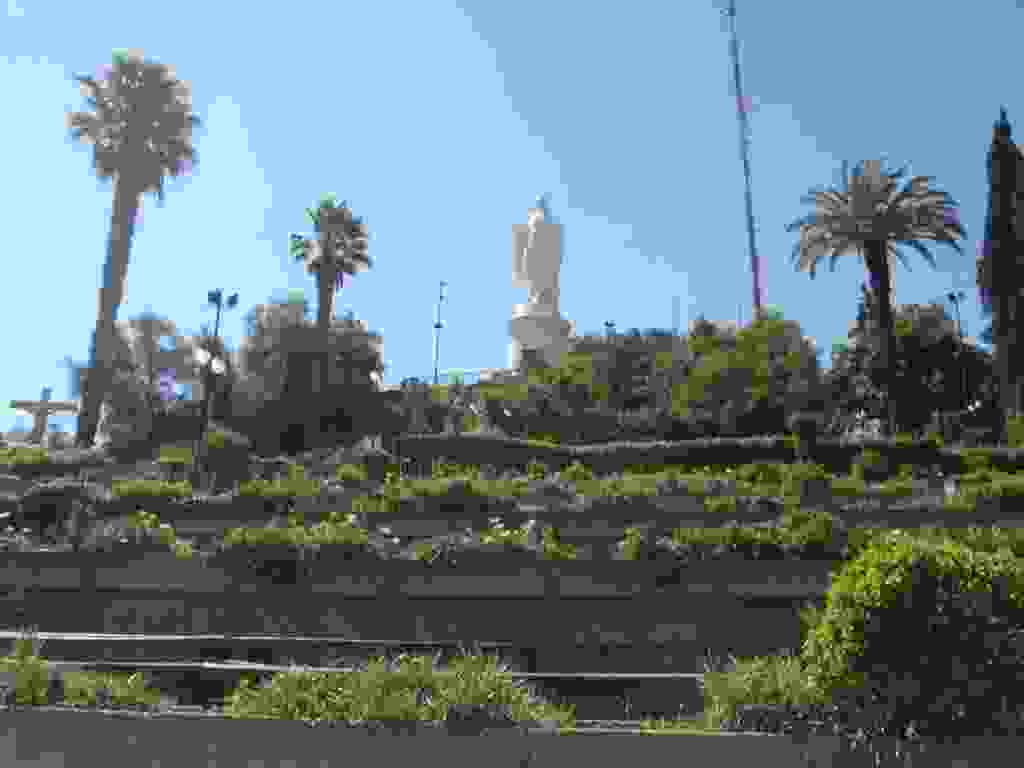
\includegraphics[height=90mm]{../wp-content/uploads/2015/03/P3052592-1024x768.jpg} } 
A côté de la grande tour, le Costanera Center, immense centre commercial. \newline
\centerline{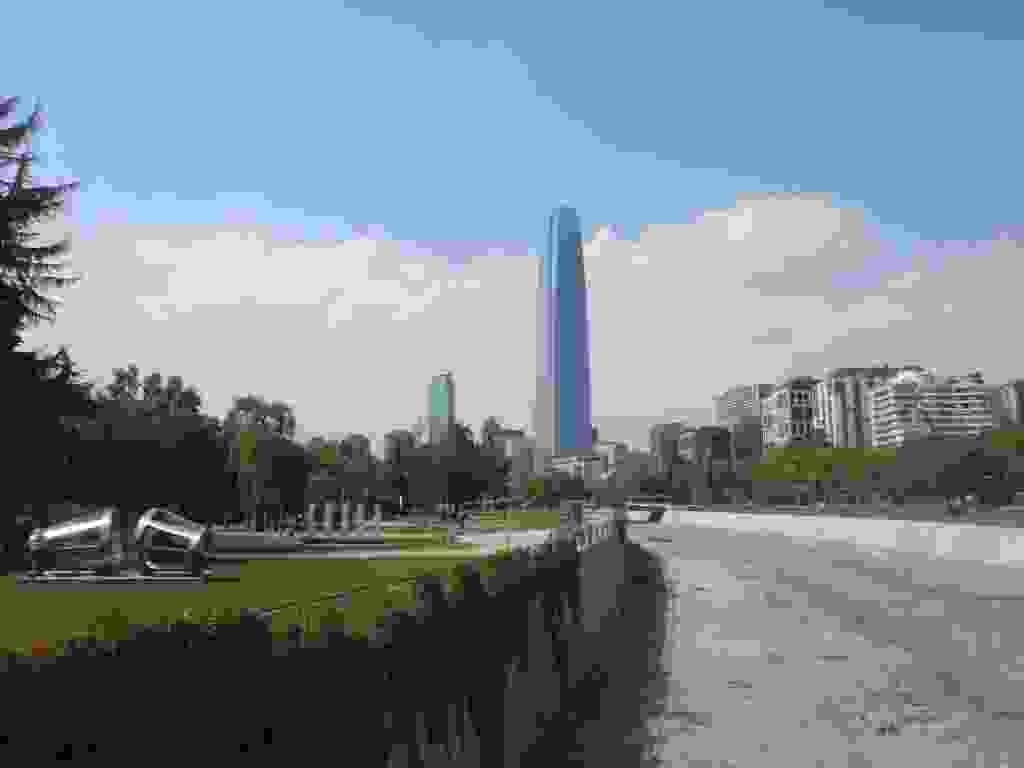
\includegraphics[height=90mm]{../wp-content/uploads/2015/03/P2282428-1024x768.jpg} } 
 \newline
\centerline{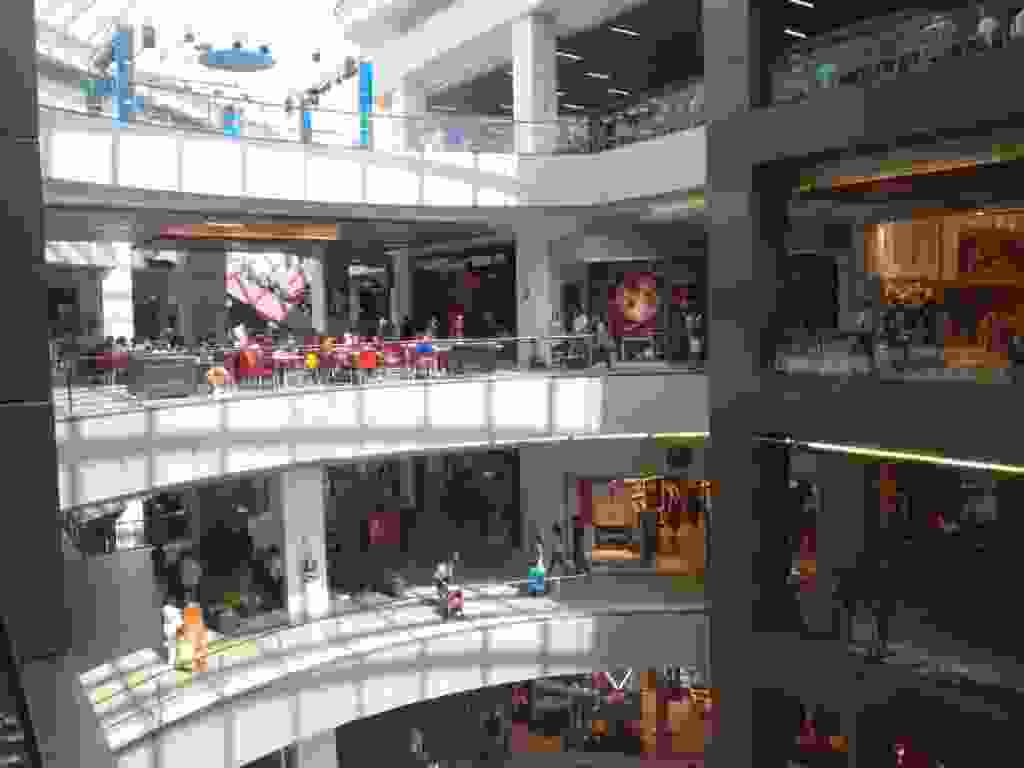
\includegraphics[height=90mm]{../wp-content/uploads/2015/03/P2282431-1024x768.jpg} } 
 Le Terremoto, cocktailtypique à base de vin blanc, jus de fruit, liqueur et glace. Très bon ! \newline
\centerline{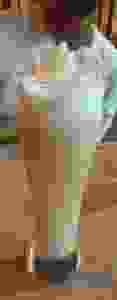
\includegraphics[height=90mm]{../wp-content/uploads/2015/03/P3062608-117x300.jpg} } 
 Dernier jour à Santiago dans un hostel qui donne directement sur la place d'armes, l'idéal ! \newline
\centerline{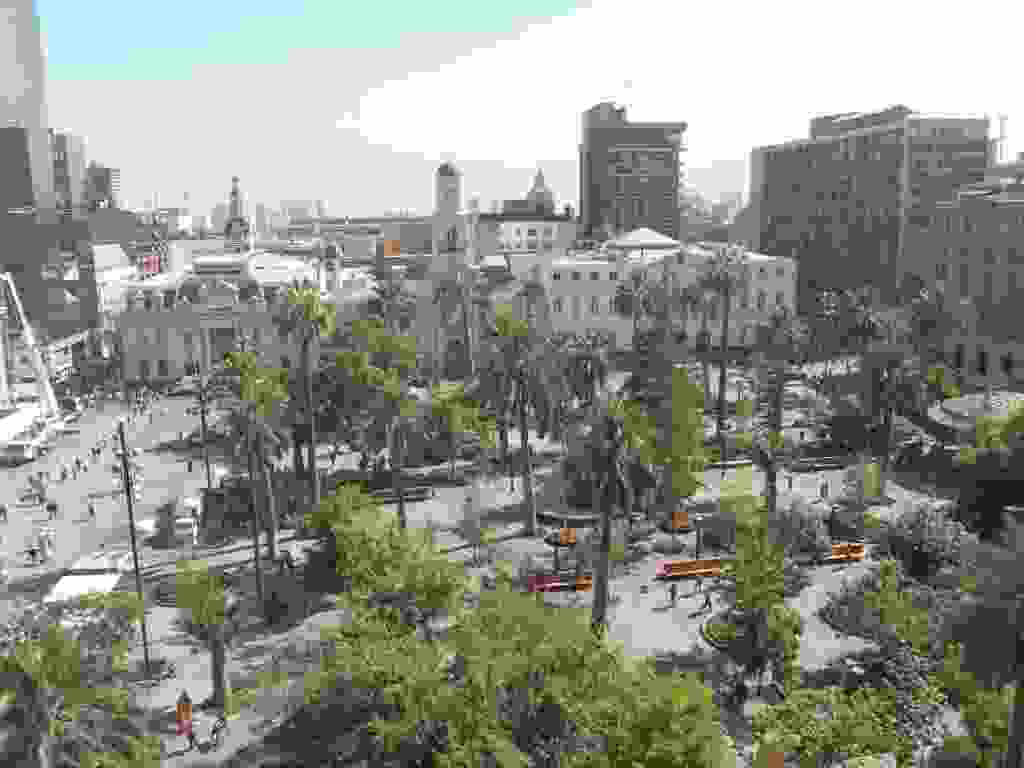
\includegraphics[height=90mm]{../wp-content/uploads/2015/03/P3062616-1024x768.jpg} } 
 \newline
\centerline{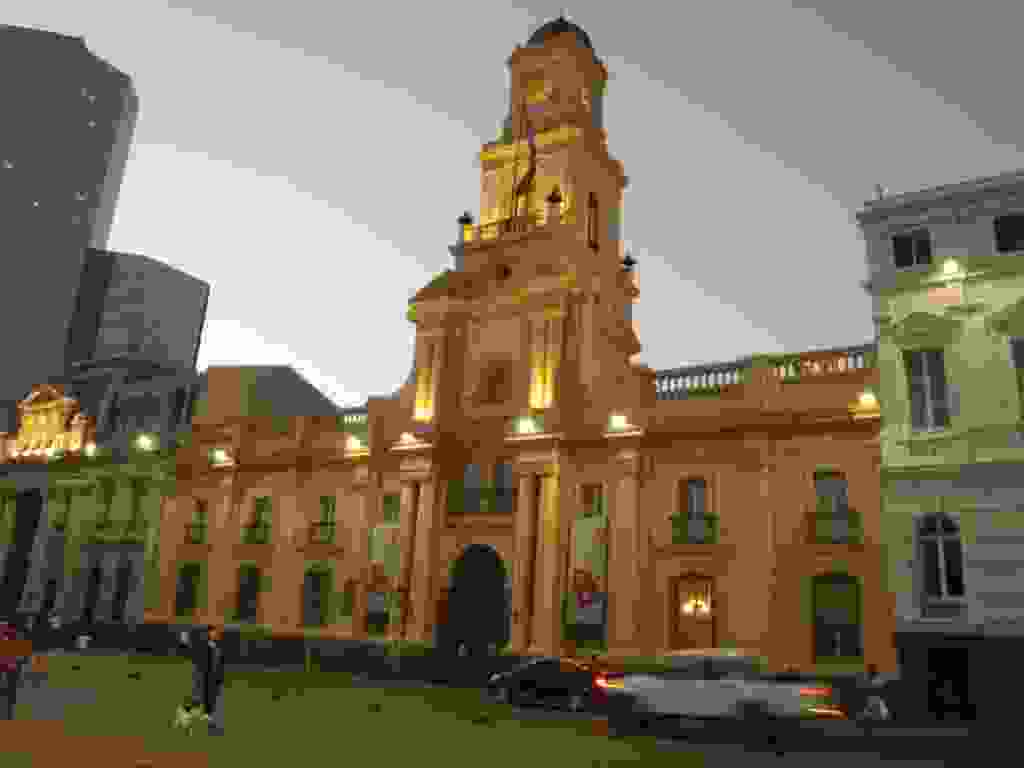
\includegraphics[height=90mm]{../wp-content/uploads/2015/03/P3062606-1024x768.jpg} } 
 \newline
\centerline{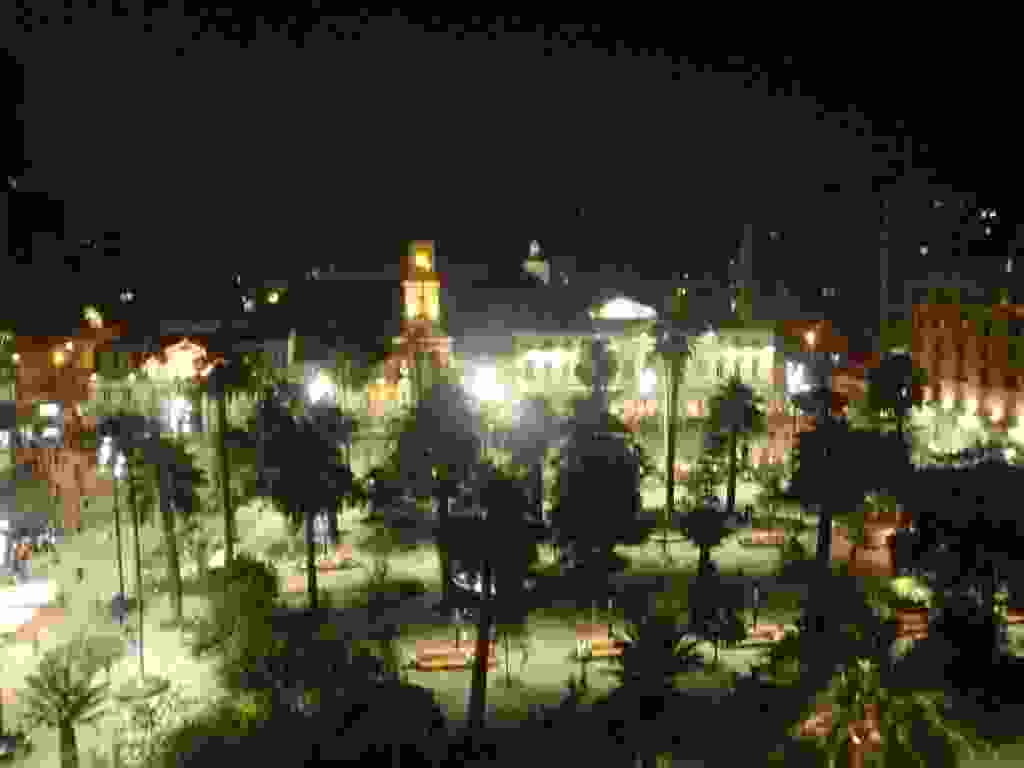
\includegraphics[height=90mm]{../wp-content/uploads/2015/03/P3072632-1024x768.jpg} } 
  La route vers Valparaiso \newline
 Après 3 jours de visite de Santiago, je remonte sur le vélo direction Valparaiso. Presque 125km par une autoroute plus ou moins agréable en vélo. La route passait par 2 tunnels interdits au vélos, heureusement le stop marche bien au Chili j'ai traversé sans trop de difficulté. \newline
 Passage par la région de Casablanca au milieu des vignes. \newline
\centerline{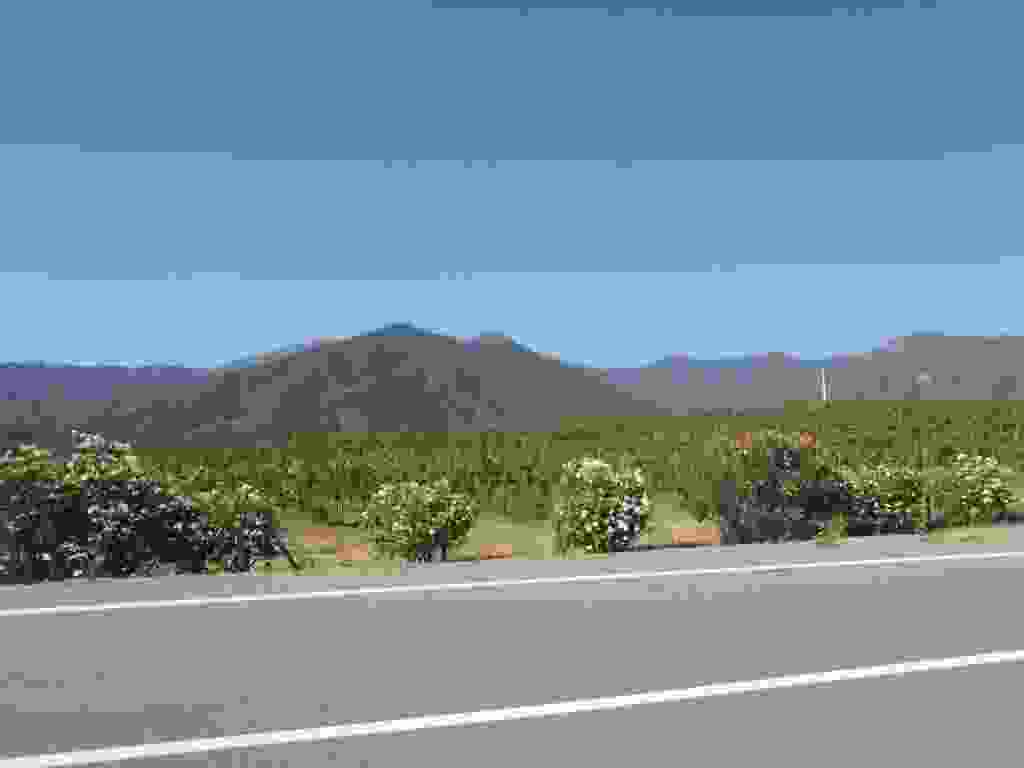
\includegraphics[height=90mm]{../wp-content/uploads/2015/03/P3072634-1024x768.jpg} } 
 \newline
\centerline{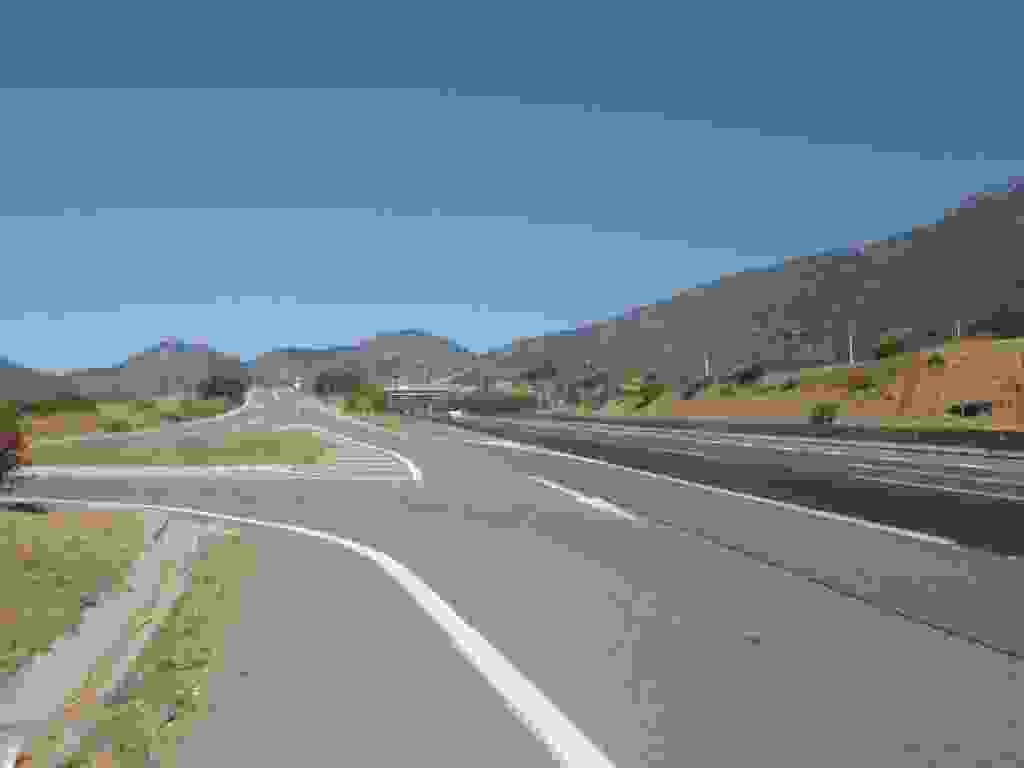
\includegraphics[height=90mm]{../wp-content/uploads/2015/03/P3072635-1024x768.jpg} } 
 \newline
\centerline{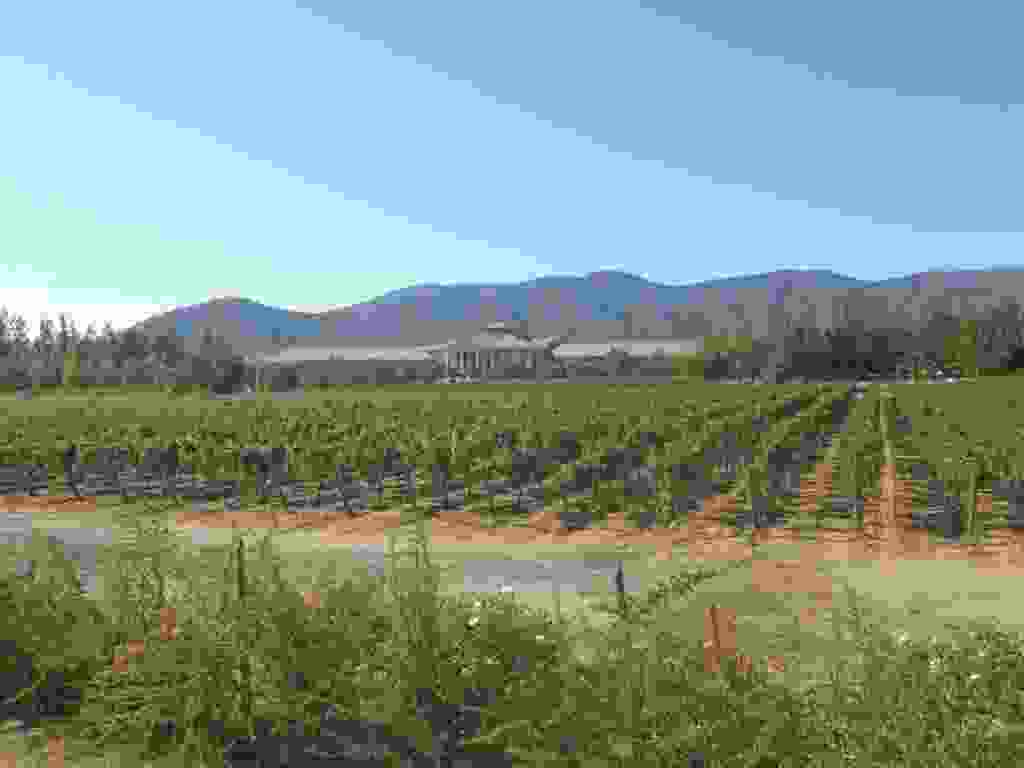
\includegraphics[height=90mm]{../wp-content/uploads/2015/03/P3072636-1024x768.jpg} } 
  Je me suis arrêté pour une petite dégustation : un syrah 2013\newline
\centerline{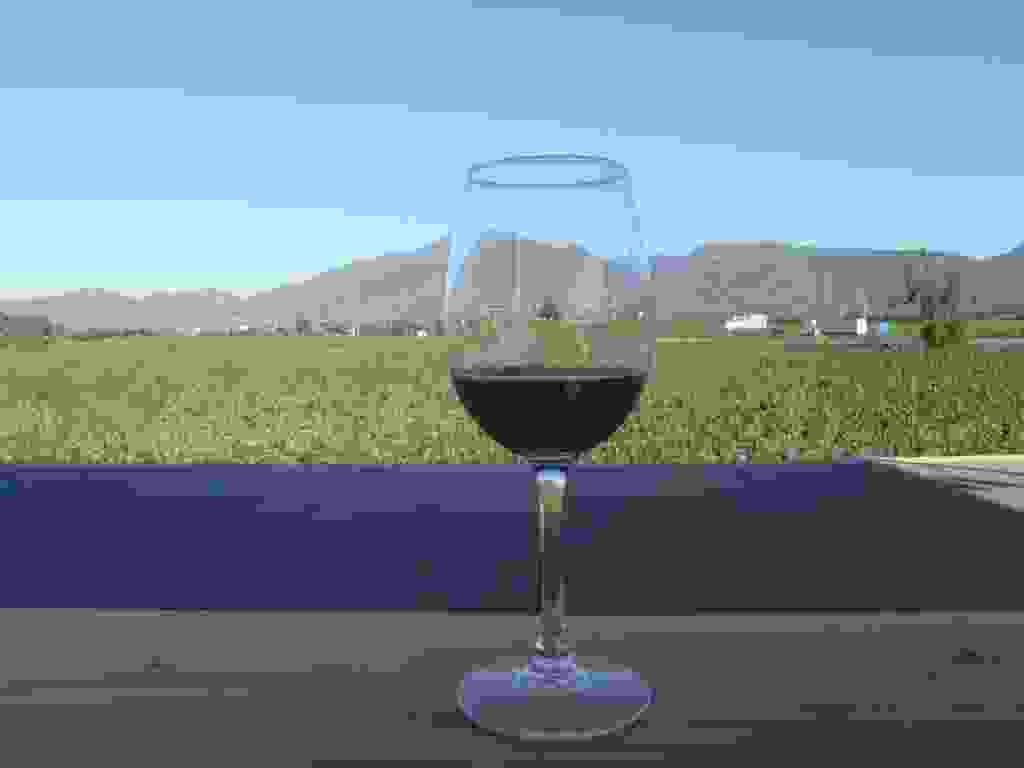
\includegraphics[height=90mm]{../wp-content/uploads/2015/03/P3072637-1024x768.jpg} } 
 \newline
\centerline{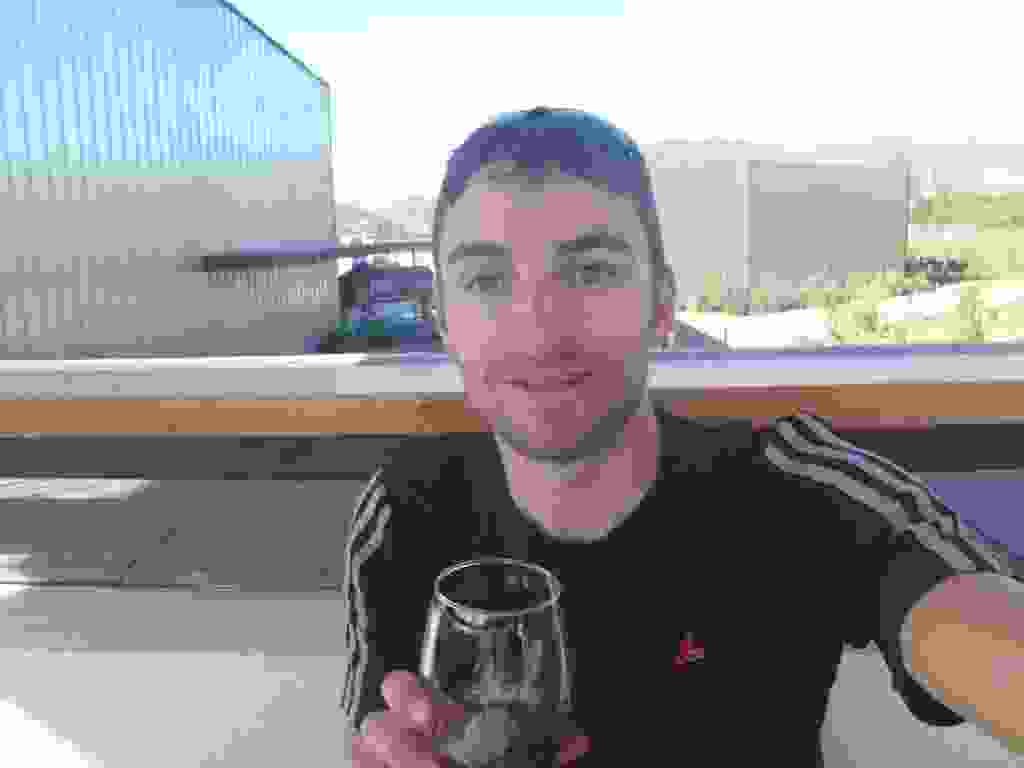
\includegraphics[height=90mm]{../wp-content/uploads/2015/03/P3072642-1024x768.jpg} } 
 \newline
\centerline{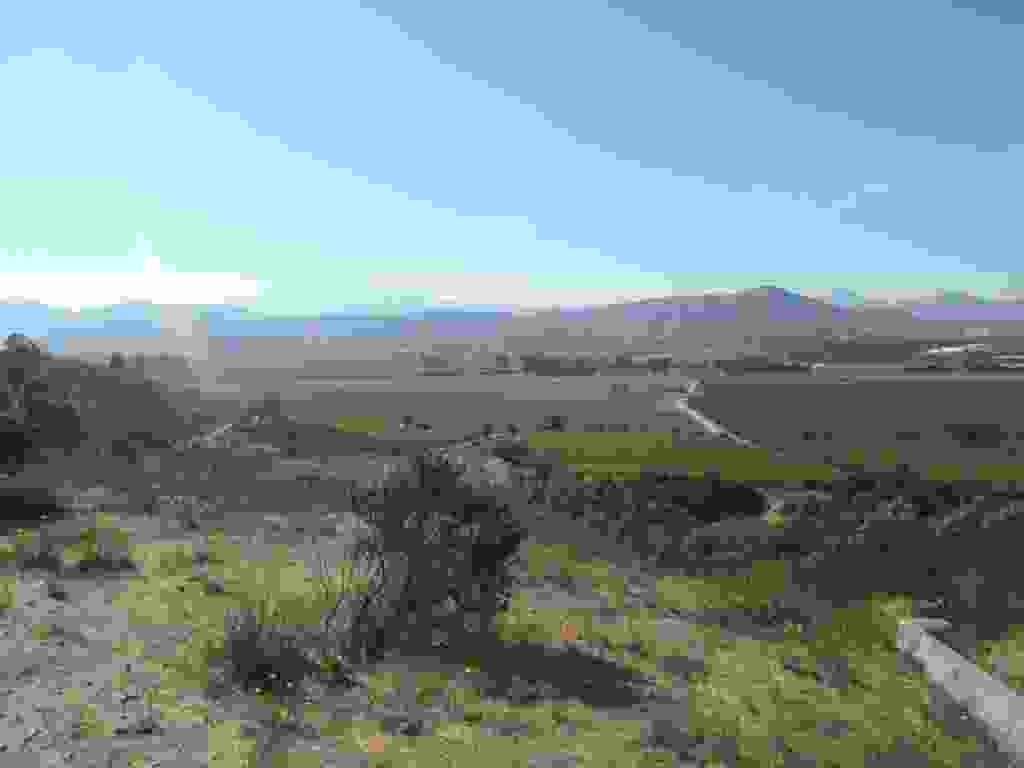
\includegraphics[height=90mm]{../wp-content/uploads/2015/03/P3082646-1024x768.jpg} } 
Avant d´arriver à Valparaiso, la Reserva Nacional Lago Peñuelas,réserve de faune et de flore autour d´un lac. \newline
\centerline{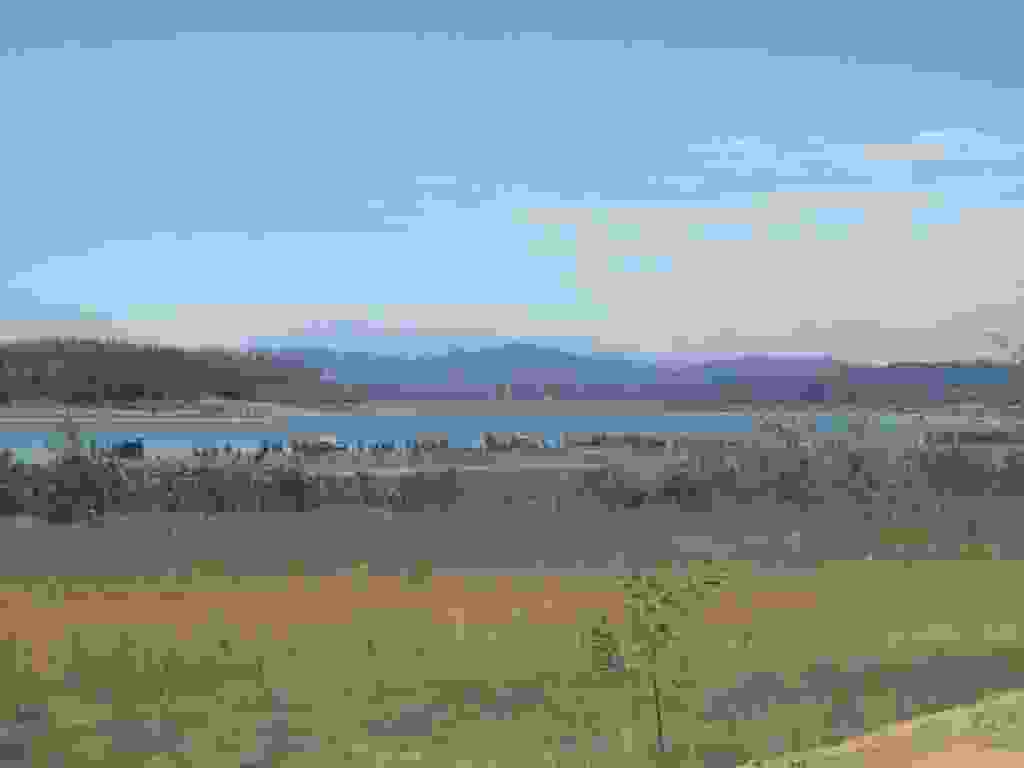
\includegraphics[height=90mm]{../wp-content/uploads/2015/03/P3082661-1024x768.jpg} } 
 \newline
\centerline{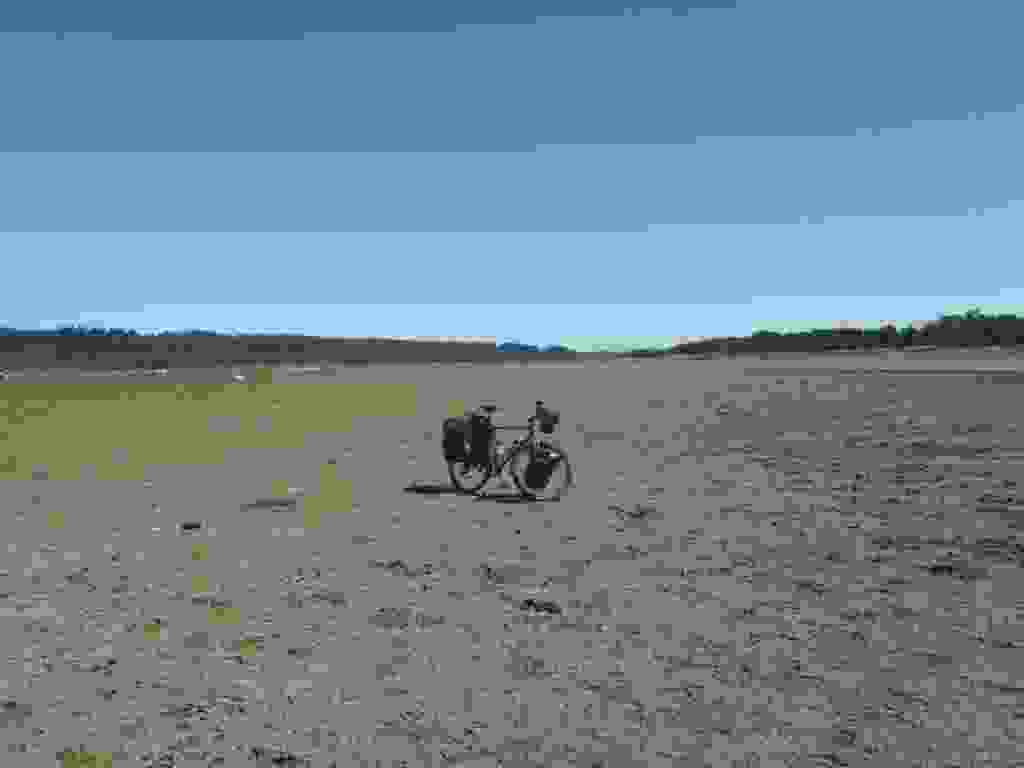
\includegraphics[height=90mm]{../wp-content/uploads/2015/03/P3082659-1024x768.jpg} } 
 Il y avait même quelques lamas. \newline
\centerline{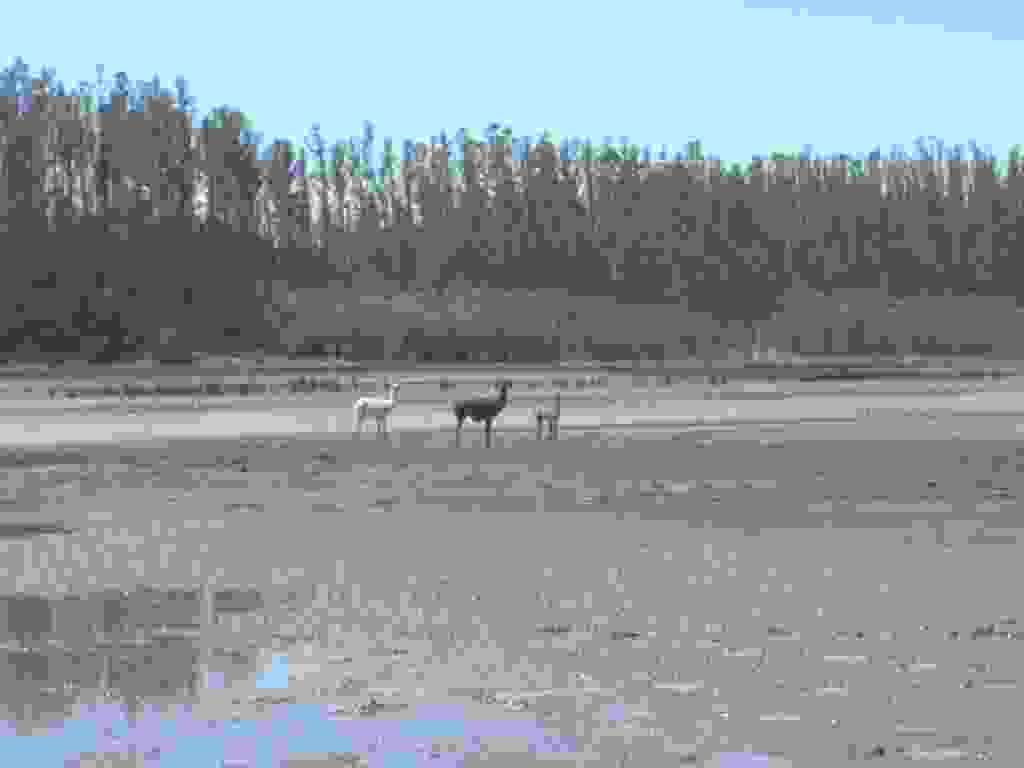
\includegraphics[height=90mm]{../wp-content/uploads/2015/03/P3082653-1024x768.jpg} } 
 \newline
\centerline{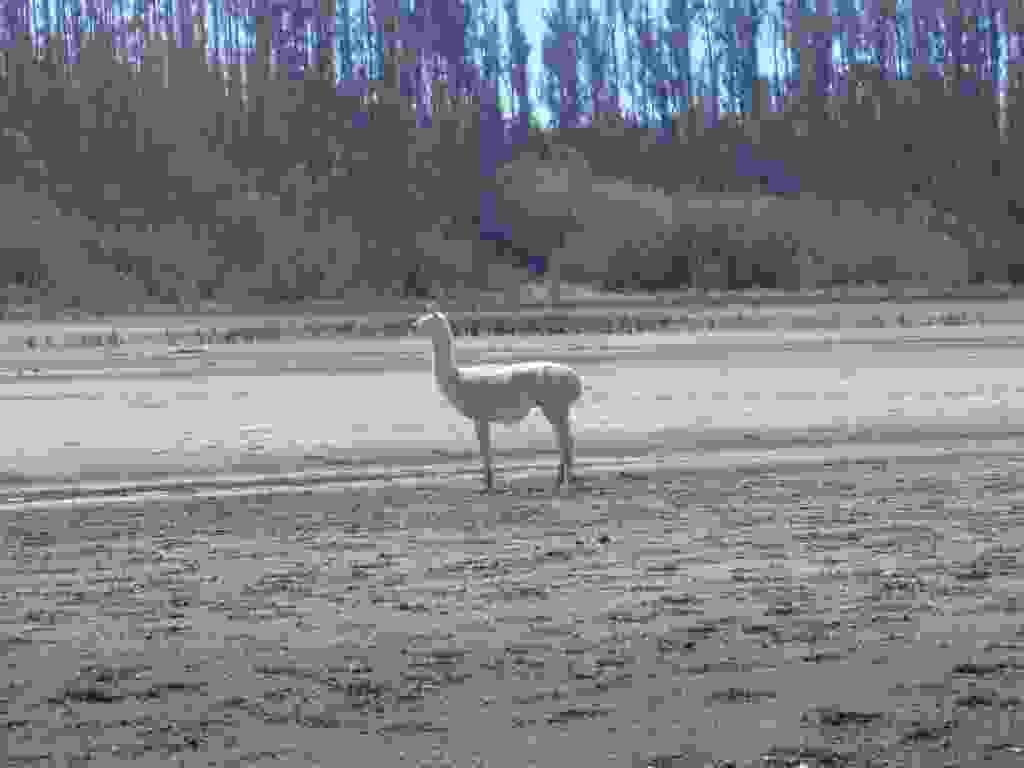
\includegraphics[height=90mm]{../wp-content/uploads/2015/03/P3082656-1024x768.jpg} } 
 \newline

\newpage
 
